%\documentclass[11pt,a4paper]{article}
\documentclass[11pt,a4paper]{book}
\usepackage[english]{babel}
\usepackage{graphicx,latexsym,isabelle,isabellesym,pdfsetup}

% proper setup for best-style documents
\urlstyle{rm}
\isabellestyle{it}

\pagestyle{myheadings}

%make a bit more space
\addtolength{\hoffset}{-1,5cm}
\addtolength{\textwidth}{3cm}
\addtolength{\voffset}{-1cm}
\addtolength{\textheight}{2cm}

\renewcommand{\setisabellecontext}[1]{\markright{Theory~#1}}

\newcommand{\secref}[1]{Section~\ref{#1}}
\newcommand{\secrefs}[1]{Sections~\ref{#1}}
\newcommand{\charef}[1]{Chapter~\ref{#1}}
\newcommand{\charefs}[1]{Chapters~\ref{#1}}

%remove clutter from the toc
\setcounter{secnumdepth}{2}
\setcounter{tocdepth}{1}

\begin{document}

\title{A Machine-Checked Model for a Java-like Language,\\
       Virtual Machine and Compiler}
\author{Gerwin Klein \and Tobias Nipkow}
\maketitle


\tableofcontents

\section{Introduction}

This document is based on
\cite{ArkoudasETAL04VerifyingFileSystemImplementationICFEM}, which
explores the challenges of verifying the core operations of a
Unix-like file system \cite{thompson78unix,mckusick84fast}.  The paper
\cite{ArkoudasETAL04VerifyingFileSystemImplementationICFEM} formalizes
the specification of the file system as a map from file names to
sequences of bytes, then formalizes an implementation that uses such
standard file system data structures as i-nodes and fixed-sized disk
blocks.  The correctness of the
implementation is verified by proving the existence of a simulation relation
\cite{RoeverEngelhardt98DataRefinement} between the specification and
the implementation.  The original effort of
\cite{ArkoudasETAL04VerifyingFileSystemImplementationICFEM} started in
Isabelle.  The process of developing the proof in Isabelle helped to 
remove the initial bugs in the concrete and
abstract models (though the proof has not been completed so far).  

Here we present a completed proof for a simplified problem:
data refinement of a single file.  We present operations on
both abstract and concrete files, define a function mapping
concrete files to abstract files, and prove that this
function is a simulation relation.

We use two libraries of arrays: arrays without bounds
checks, which can be thought of as an array with an
unbounded number of elements, and resizable arrays, which
have a notion of the current size, but expand in response to
array writes that are outside the current bounds.


\section{Theory Dependencies}

Figure \ref{theory-deps} shows the dependencies between 
the Isabelle theories in the following sections.

\begin{figure}[h!t]
\begin{center}
  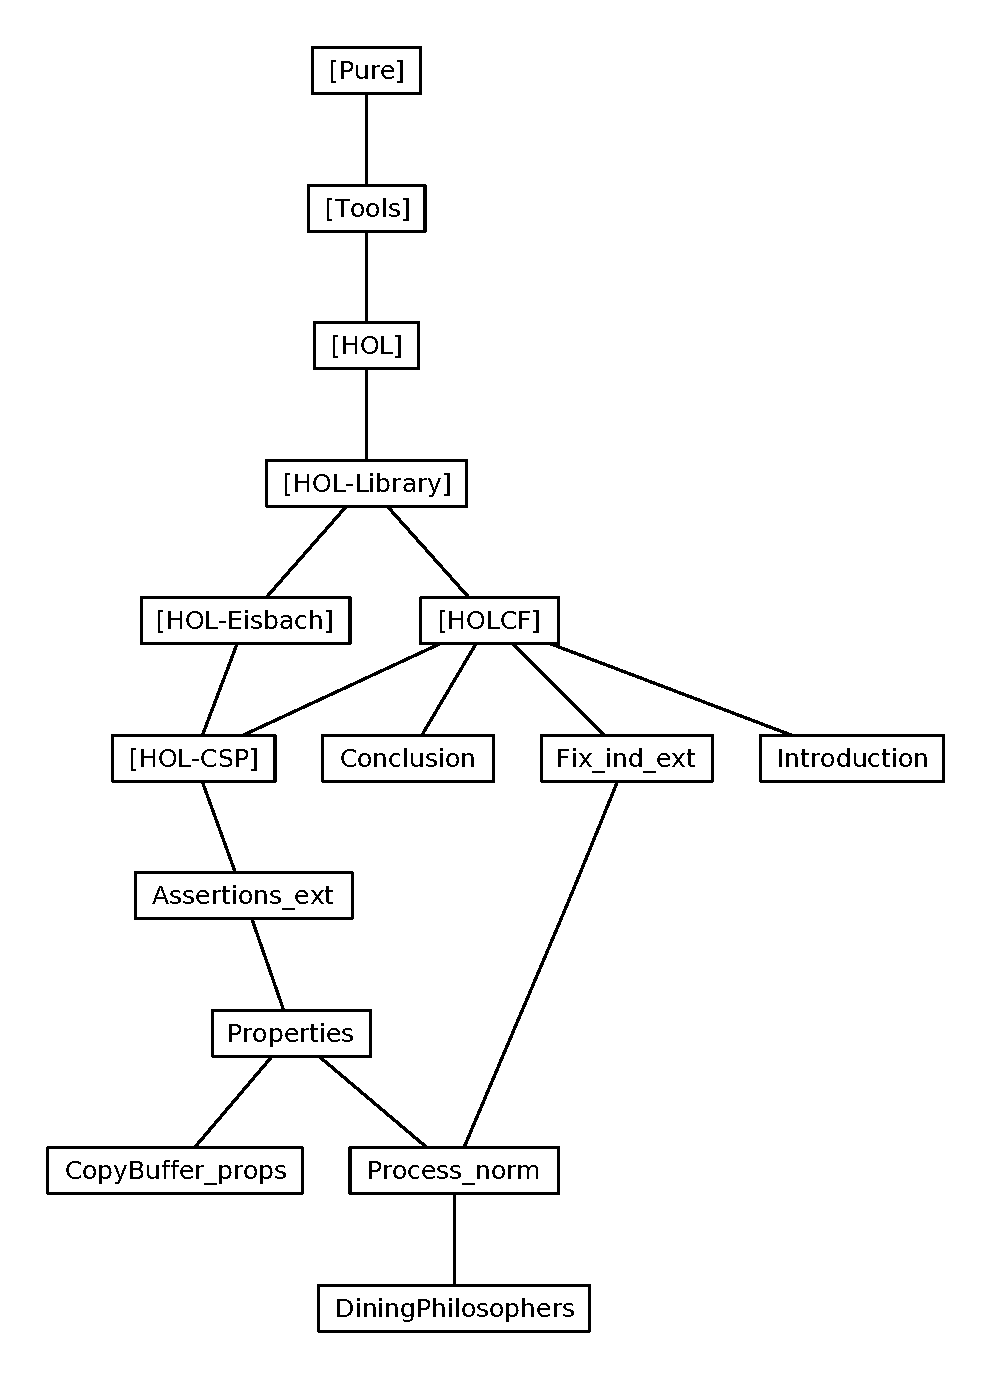
\includegraphics[width=\textwidth]{session_graph}
\end{center}
\caption{Theory Dependency Graph\label{theory-deps}}
\end{figure}

\newpage
\input{session}

\newpage
\nocite{*}
\bibliographystyle{abbrv}
\bibliography{root}

\end{document}
